\documentclass[twocolumn,floatfix,nofootinbib,aps]{revtex4-1}
\usepackage[utf8]{inputenc}

\usepackage{algorithmicx, algpseudocode, algorithm}
\usepackage{amsmath}    % need for subequations
\usepackage{amssymb}    % for symbols
\usepackage{graphicx}   % need for figures
\usepackage{verbatim}   % useful for program listings
\usepackage{color}      % use if color is used in text
\usepackage{subfigure}  % use for side-by-side figures
%\usepackage{hyperref}   % use for hypertext links, including those to external documents and URLs

% new commands
\DeclareMathOperator*{\argmax}{argmax\,}
\renewcommand{\vert}{\, | \,}

\usepackage[capitalise]{cleveref}   % use for referencing figures/equations
\begin{document}
\title{Notes on Simulating Mutants: Efficient MSM-based Sampling Strategies}
\author{Robert T. McGibbon}

\begin{abstract}
\end{abstract}
\maketitle

\section{Introduction}
Mutational analysis is one of the central tools in experimental protein science, but remains a challenge for simulation. Using standard simulation
approaches, the study of a protein and a single mutant requires 2x the computational effort of studying just the original protein. Can we use MSMs to do better?

Assume that we've run extensive, converged simulation of a protein, $A$, and we build an MSM. We now want to run a mutant, $A'$. We assume that $A$, and $A'$ share a common state space -- the interest is in how the mutation affects
the transition probabilities.

If we assume that the mutation affects the transition matrix in a ``small'' way -- that the mutation is appropriately classified as a perturbation, then it should be possible to ``win''. First, short trajectories (of length equal to a single lag-time) are sufficient, because (by assumption), we don't have to discover any new states. We just have to estimate the perturbed transition probabilities. Second, because the mutation is small, there's a lot of mutual information between transition probabilities in $A$ and those in $A'$. We're not starting from scratch here.

\section{Problem Statement}
What is the mathematical model for the cross-talk between $A$ and $A'$? Our observation of $A$ must basically be the prior for $A'$.

Consider a row of the transition matrix $T^{A'}$, the transition probabilities
leaving state $i$, $\vec{p}_i^{A'}$. In the absence of any simulation data on $A'$, what is our prior distribution on $P(\mathbf{p_i}^{A'})$?

The simplest idea is that the $\vec{p}_i^{A'}$ are $\operatorname{Dir}(\mathbf{\alpha})$, where the $\mathbf{\alpha}$ parameters (effectively the psuedocounts) are determined by the number of observed counts in protein $A$, $\vec{c}_i^A$. If there is a lot of mutual information between $A$ and $A'$, then the $\alpha$ should be equal to $\vec{c}_i^A$. This formalizes the idea that our predictions about protein $A'$ made from data collected on $A$ are equally confident as our predictions about protein $A$ using the same data collected on $A$. But if there's not a lot of mutual information between the two proteins, then our prior on $\vec{p}_i^{A'}$ should be non-informative.

$$
\vec{p}_i^{A'} \sim \operatorname{Dir}(q_i \cdot \vec{c}_i^A + 1/2)
$$

Here, the parameter $q_i \in [0,1]$ gives something like the expected strength of the information transfer between state $i$ in the the two models. When $q_i=1$, a count measured in $A$ is ``worth it's weight'' in the $A'$ model. But as $q_i \rightarrow 0$, those counts are worthless in $A'$ and we get a noninformative Jeffreys prior.

This statement of the problems is nice because it takes into account some uncertainty in the gold-standard model for $A$. It doesn't just look the MLE estimate of the transition matrix in $A$, but uses the counts directly to parameterize the distribution over $A'$. So for regions of the state space where $\vec{c}_i^{A'}$ is low, we're going to get a mostly uninformative prior naturally.

One question: should $q$ be a single parameter for the whole model, or should every state have its own $q_i$? The later case could encode the idea that some of the states behave very similarly in $A$ vs. $A'$, whereas other might be very different.

Next: clearly $q_i$ should not be a fixed parameter. It should also be a random variable, estimated from the data. Perhaps the appropriate prior on $q_i$ is $q_i \sim \operatorname{Beta}(\alpha, \beta)$.

Now, if observe some outbound counts, $\vec{K}$, from state $i$ in simulations of the mutant protein $A'$ (note for consistency, we could notate $\vec{K}$ as $\vec{c}_i^{A'}$ instead), they are distributed as a multinomial with parameters $\vec{p}_i^{A'}$. The model specified is then:
 
\begin{align*}
    \vec{c}_i^A &= \text{prior observed counts in protein $A$}\\
    \alpha, \beta &= \text{$q$'s hyperparameters}\\
    q_i &\sim \operatorname{Beta}(\alpha, \beta) \\
    \vec{p}_i^{A'} &\sim \operatorname{Dirichlet}(q \cdot \vec{c}_i^A + 1/2)\\
    K &\sim \operatorname{Multinomial}(\vec{p}_i^{A'})
\end{align*}

Can we do inference here? I think so. Let's start with the joint distribution of of $\vec{p}_i^{A'}$ and $q_i$. By bayes rule,

$$
P(q_i, \vec{p}_i^{A'} \vert \vec{K}) \propto P(\vec{K} \vert q, \vec{p}_i^{A'}) \;  P(q_i, \vec{p}_i^{A'})
$$

$K$ is conditionally independent of $q_i$ given $\vec{p}_i^{A'}$, and is multinomial. $P(q_i, \vec{p}_i^{A'})$ factors as $P(\vec{p}_i^{A'} \vert q_i) \cdot  P(q_i)$, a Dirichlet times a Beta. Because of the conjugacy, $P(\vec{K} \vert q_i, \vec{p}_i^{A'})$ and $P(\vec{p}_i^{A'} \vert q_i)$ group together into an updated Dirichlet. Putting it all together, we get

$$
P(q_i, \vec{p}_i^{A'} \vert \vec{K}) \propto \operatorname{Dir}(q_i \cdot \vec{c}_i^{A} + \vec{K} + 1/2) \cdot P_{\alpha, \beta}(q)
$$

And then marginalizing out $q_i$, we have


$$
P(\vec{p}_i^{A'} \vert \vec{K}) \propto \int_0^1 dq \; \operatorname{Dir}(q \cdot \vec{c}_i^{A} + \vec{K} + 1/2) \cdot  P_{\alpha, \beta}(q_i)
$$



%With MCMC, I think sampling from this posterior is pretty straightforward. But what about an analytic solution? When I write out the integral explicitly, it looks pretty bad.

%\begin{align*}
%P(\vec{p}_i^{A'} &= \vec{x} \vert \vec{K}) \propto \int_0^1 dq \; \frac{1}{Z(q_i)} \prod_{j=1} x_j^{q_i \cdot \vec{c}_{ij}^{A'} + \vec{K}_j + 1/2} q_i^{\alpha-1}(1-q_i)^{\beta-1}\\
%Z(q_i) &= \frac{1}{B(q \cdot \vec{c}_i^{A} + \vec{K} + 1/2) \cdot B(\alpha, \beta)}
%\end{align*} 

%But if instead we knew $q$ directly -- i.e. by just fixing at a certain value, then the distribution for $P(\vec{p}_i^{A'})$ would be simple. Maybe we do MCMC to sample over $q$, and then use analytic formulas given $q$...

\section{Active Learning}
We've done a little bit of simulation in $A'$, and now we want to start some new simulations. From which state $i$ should we start our next round of sampling?

The goal should be, in some sense, to maximize our expected information gain, or achieve the greatest reduction in the model's uncertainty. We consider two strategies alternative.

\subsection{Maximize Information Gain in Transition Probabilities}

First, we consider adaptively choosing the state from which to start new simulations in a way that maximizes the expected information gain in the transition probabilities $p_{ij}$. Conditional on $q_i$, the expected information gain in the outbound transition probabilities from state $i$ is given by the expected Kullback–Leibler divergence between the current
$P(p_i^{A'})$ and the updated posterior, $P(p_i^{A'} | e)$, where $e$ is newly observed transition, distributed according to the current model.

The K-L divergence from one Dirichlet distribution, $p$, to another, $q$, is given by

\begin{align*}
D_{KL}(\lambda^q || \lambda^p) = \log& \frac{\Gamma(\lambda^{qt})}{\Gamma(\lambda^{pt})} + \sum_{s=1}^m \log \frac{\Gamma(\lambda^p_s)}{\Gamma(\lambda^q_s)} \\
&+ \sum_{s=1}^m \left[\lambda^q_s -\lambda^p_s\right]\left[\Psi(\lambda^q_s) - \Psi(\lambda^{qt})\right]
\end{align*}

Where $\lambda^p$ and $\lambda^q$ are the parameters of the two Dirichlet distributions, $\lambda^{qt} = \sum_{s=1}^{m}\lambda^q_s$, $\lambda^{pt} = \sum_{s=1}^{m}\lambda^p_s$, and $m$ is the number of states.

If $\lambda^p$ is formed from $\lambda^q$ by incrementing a single element $l$  by one, then by simple properties of the gamma function, it can be shown that

\begin{align*}
D_{KL}(\lambda || \lambda + e_l) = - \log(\lambda^t) + \log(\lambda_l) + \Psi(\lambda^{t}) - \Psi(\lambda_l)
\end{align*}

Then, the expected KL divergence is 

$$
E[D_{KL}] = \sum_l D_{KL}(\lambda || \lambda + e_l) P(l | \lambda)
$$

$P(l \vert \lambda) = \int d \vec{p} \; P(l \vert \vec{p}) P(\vec{p} \vert \lambda)$ follows the Multinomial-Dirichlet distribution, with $P(l \vert \lambda) = \lambda_l / \lambda^t$. Thus the expected information gain comes out to be

$$
E[D_{KL} \vert q_i] = \Psi(\lambda^t) - \log(\lambda^t) + \frac{1}{\lambda^t} \sum_l \left[ \lambda_l \left( \log (\lambda_l) - \Psi(\lambda_l) \right) \right] 
$$

This formula is still conditional on $q_i$. Thus the procedure is to fit the model for each row of the transition matrix with MCMC and then compute, for each sampled $\lambda$ from the posterior, the expected information gain as above. The mean over the samples is then the final ``score'' for each state. At each step we choose the to initialize new sampling from the state with the highest such score.

\begin{figure*}[h]
\centering
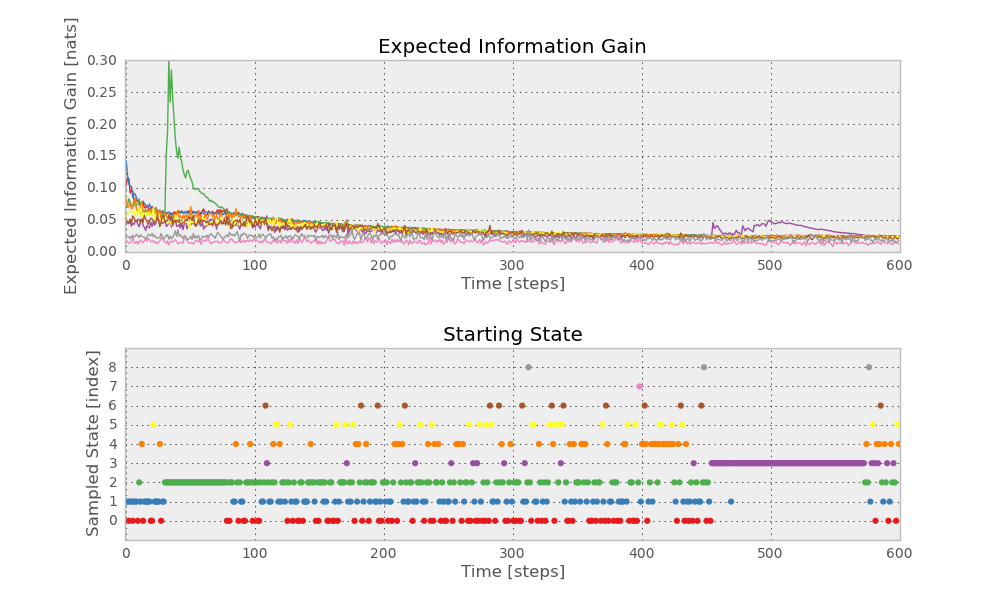
\includegraphics[width=7in]{../code/9x9graph/plots/information_gain.png}
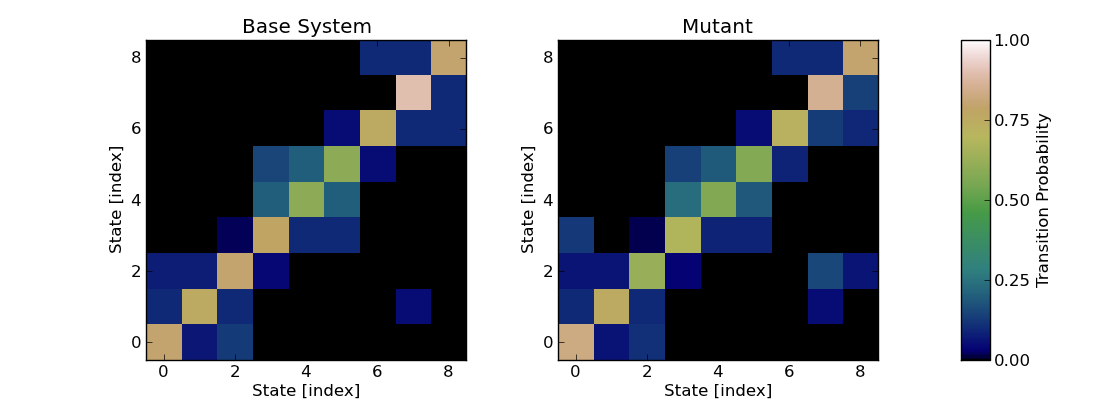
\includegraphics[width=7in]{../code/9x9graph/plots/transition_matricies.png}
\caption{Sampling a nine state transition matrix by maximizing the expected information gain. The top two panels show the progress of the sampling, with the expected information gain at each step in the upper panel, and the chosen state in the second panel. On the bottom, the base and mutant transition matrices are shown. The base counts were generated from contiguous 5000 step trajectory. The two peaks in the expected information gain show the sampler effectively discovering the mutations in states two and three, and the effectively focusing its sampling on those states for a period of time.}
\end{figure*}

\begin{figure*}[h]
\centering
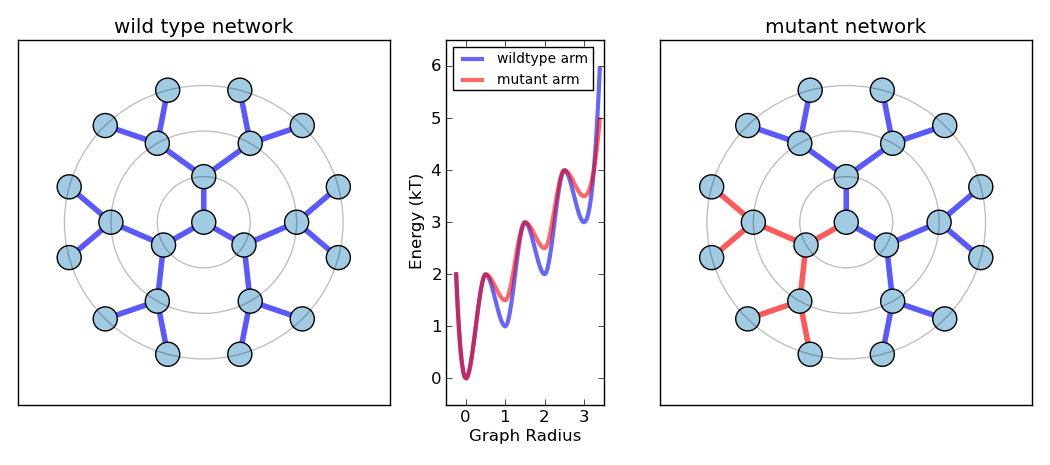
\includegraphics[width=7in]{../code/cayleytree/figures/cayley.png}
\caption{Cayley tree toy model, in which a mutation destabilizes one of the ``arms'' of the network. The system was constructed via a rate matrix construction.}
%\caption{Sampling a nine state transition matrix by maximizing the expected information gain. The top two panels show the progress of the sampling, with the expected information gain at each step in the upper panel, and the chosen state in the second panel. On the bottom, the base and mutant transition matrices are shown. The base counts were generated from contiguous 5000 step trajectory. The two peaks in the expected information gain show the sampler effectively discovering the mutations in states two and three, and the effectively focusing its sampling on those states for a period of time.}
\end{figure*}

\subsection{Minimize Uncertainty in the First Eigenvalue}

The procedure above treats the entropy in each row of the transition matrix independently and on equal footing. But if we care about predicting the long-time dynamics of the system accurately, we care substantially more about some states than others.

Instead of maximize the information gain in the transition probabilities, $p_{ij}$, an alternative would be to minimize the uncertainty in the model's longest implied timescale.

\section{Limitations and Future Work}
While the framework presented in this paper is powerful, it neglects some key aspects of the adaptive sampling problem. First, the because the number of states is fixed by the model, the expected information gain formalism is unable to reason about the probability of discovering a new state. For the mutant problem, we thus rely on the proposition that the ``base'' sampling discovered all of the states. In order to properly address possibility of state discovery in the Bayesian framework, we would need to switch to a non-parametric framework, for instance based on the Dirichlet process.

Reversibility is not dealt with.

What about other ideas of how mutants act? For instance, a reasonable hypothesis is that they destabilize/stabilize a state. So, perhaps its metastability changes, but the ratio of the outbound transition probabilities change less so. This could be incorporated into the model, instead of, or in addition to, $q$.

\end{document}